%  LaTeX support: latex@mdpi.com
%  In case you need support, please attach any log files that you could have,
% and specify the details of your LaTeX setup (which operating system and LaTeX
% version / tools you are using).

%=================================================================

% LaTeX Class File and Rendering Mode (choose one)
% You will need to save the "mdpi.cls" and "mdpi.bst" files into the same folder
% as this template file.

%=================================================================

\documentclass[energies,article,accept,moreauthors,pdftex,12pt,a4paper]{mdpi}

%=================================================================
\setcounter{page}{1}
\lastpage{x}
\doinum{10.3390/------}
\pubvolume{xx}
\pubyear{2015}
\history{Received: xx / Accepted: xx / Published: xx}
%------------------------------------------------------------------
% The following line should be uncommented if the LaTeX file is uploaded to
% arXiv.org
%\pdfoutput=1

%=================================================================

% Add packages and commands to include here
% The amsmath, amsthm, amssymb, hyperref, caption, float and color packages are
% loaded by the MDPI class.
\usepackage{graphicx}
%\usepackage{subfigure,psfig}
\usepackage[draft]{todonotes}
\usepackage{lineno}

\def \p{\partial}
\def \d{\mathrm{d}}
\def \D{\mathrm{D}}

%=================================================================
%% Please use the following mathematics environments:
%\theoremstyle{mdpi}
%\newcounter{thm}
%\setcounter{thm}{0}
%\newcounter{ex}
%\setcounter{ex}{0}
%\newcounter{re}
%\setcounter{re}{0}
%\newtheorem{Theorem}[thm]{Theorem}
%\newtheorem{Lemma}[thm]{Lemma}
%\newtheorem{Characterization}[thm]{Characterization}
%\newtheorem{Proposition}[thm]{Proposition}
%\newtheorem{Property}[thm]{Property}
%\newtheorem{Problem}[thm]{Problem}
%\newtheorem{Example}[ex]{Example}
%\newtheorem{Remark}[re]{Remark}
%\newtheorem{Corollary}[thm]{Corollary}
%\newtheorem{Definition}[thm]{Definition}
%% For proofs, please use the proof environment (the amsthm package is loaded by
% the MDPI class).

%=================================================================

% Full title of the paper (Capitalized)
\Title{Effects of Reynolds Number on the Energy Conversion and Near-Wake Dynamics of a
High Solidity Vertical-Axis Cross-Flow Turbine}

% Authors (Add full first names)
\Author{Peter Bachant $^{1,}$* and Martin Wosnik $^{1}$}

% Affiliations / Addresses (Add [1] after \address if there is only one
% affiliation.)
\address{%
$^{1}$ Center for Ocean Renewable Energy, University of New Hampshire, 24
Colovos Rd., Durham, NH, USA}

% Contact information of the corresponding author (Add [2] after \corres if
% there are more than one corresponding author.)
\corres[2]{pxL3@unh.edu, martin.wosnik@unh.edu}

% Abstract (Less than 200 words)
\abstract{The performance and wake characteristics of cross-flow (vertical axis)
    turbines depend on many parameters: solidity, blade profile, blade pitch, number
    of blades, strut drag, operational parameters such as tip speed ratio---and
    Reynolds number. Tolerable mismatch between physical model Reynolds number and
    full-scale Reynolds number was investigated from both the perspective of
    predicting full scale performance and flow dynamics, as well as numerical model
    validation. Experiments were performed with a large laboratory-scale cross-flow
    turbine of to investigate Reynolds number dependence of performance and wake
    transport characteristics, and to determine what an acceptable Reynolds number
    mismatch is for scaled physical model tests of cross-flow turbines. It was
    demonstrated that the performance of the cross-flow turbine becomes essentially
    $Re$-independent at a Reynolds number based on turbine diameter of $Re_D \approx
    10^6$, or an approximate Reynolds number based on blade chord of $Re_c \approx 2
    \times 10^5$. A simple model that calculates peak torque coefficient from static
    foil data and cross-flow turbine kinematics was shown to be a reasonable
    estimator for predicting Reynolds number dependence of an actual cross-flow
    turbine operating under dynamic conditions.}

% Keywords: add 3 to 10 keywords
\keyword{Reynolds number; cross-flow turbine; turbine performance; marine
hydrokinetic energy; wind energy}

% The fields PACS, MSC, and JEL may be left empty or commented out if not
% applicable
%\PACS{}
%\MSC{}
%\JEL{}

\begin{document}
%\linenumbers
\listoftodos


\section{Introduction}

Scaled physical models are often used in science and engineering to approximate
real-world systems. The principle of dynamic similarity allows for geometrically
scaled systems to be dynamically identical in scale if certain nondimensional
physical parameters are matched. In the case of fluid systems, the most
important nondimensional parameter is often the Reynolds number, which
quantifies the importance of inertial forces over viscous forces on the flow
physics. It should be noted that in general the geometric scale of a physical
model is not necessarily the same as its dynamical scale. As such, hereafter we
will use the word ``scale'' to refer to this dynamical scale rather than the
geometric scale.

With regards to wind and marine hydrokinetic (MHK) turbines, scaled physical
models are used to validate predictive numerical models, predict full-scale
performance of individual turbines, and design or investigate arrays of devices.
Scaled models have the benefit of being significantly less expensive, however,
there still is concern at which scale an experiment must be performed to be
relevant to full-scale application. This is particularly important for
cross-flow turbines, where Reynolds number effects for experiments conducted at
low $Re$ are often difficult to distinguish from the effects on performance of
several other turbine parameters.

The performance and wake characteristics of cross-flow (vertical-axis) turbines
depend on turbine solidity, blade profile (lift/drag, dynamic stall at reduced
frequency of turbine rotation, symmetry, thickness, camber), blade pitch, number
of blades, strut drag and operational parameters such as tip speed ratio---{\em
    and} on Reynolds number. Note that an average blade chord Reynolds number,
$Re_{c,\mathrm{avg}} \approx \lambda U_\infty c/ \nu$, can be expressed in terms
of tip speed ratio $\lambda \equiv \omega R/ U_\infty$; the value of $\lambda$
at which a turbine reaches peak performance is again a function of turbine
solidity $Nc/\pi D$.

If numerical models are validated with physical model data that was obtained at
insufficiently high Reynolds numbers, it cannot be determined whether problems
with model predictions are caused by Reynolds number effects, other turbine
parameters or issues with the numerical model. One might also obtain different
predictions of scaled systems due to modified physics at lower Reynolds numbers,
e.g., laminar boundary layers and transitional flow regimes. If the numerical
model is then considered ``validated,'' there is a risk that its application at
full-scale may produce incorrect predictions. It is uncertain whether numerical
models validated with physical model data obtained at low Reynolds number should
be considered validated at all, since the scale at which the model will be
applied is orders of magnitude larger.

This can be overcome by showing that a scaled physical model test has become
Reynolds number independent, and therefore validation efforts should be relevant
at full-scale.  For scaled physical models, it is of interest how small---since
size, or scale generally correlates inversely with cost---the model can be while
remaining a reliable predictor of full-scale behavior. At the very least, it is
necessary to test at a scale where results can be extrapolated, i.e., changes
are occurring quasi-linearly without dramatic changes in the underlying physical
principles governing the behavior of interest, e.g., power production in the
case of a wind or MHK turbine.

Blackwell et al. investigated the effects of Reynolds number on the performance
of a 2 m diameter Darrieus vertical-axis cross-flow wind turbine with NACA 0012
blades \cite{Blackwell1976}. By varying wind tunnel speed, the turbine was made
to operate at approximately constant blade chord Reynolds number $Re_c$ ranging
from $1 \times 10^5$ to $3 \times 10^5$. In this regime the turbine power
coefficient $C_P$ was shown to be sensitive to $Re_c$, with sensitivity
diminishing at the higher Reynolds numbers, especially for turbines of lower
solidity ($Nc/R$, where $N$ is the number of blades and $R$ is the turbine's
maximum radius). More recently, Polagye and Cavagnaro observed significant
Reynolds number sensitivity for a high solidity helical cross-flow turbine
\cite{Polagye2013b}, and Bravo et al. observed power coefficient of a
straight-bladed VAWT to become Reynolds number independent at $Re_c \approx 4
\times 10^5$ \cite{Bravo2007}.

The wake of a cross-flow turbine in dynamic stall has been studied via laser
Doppler velocimetry by Brochier et al. \cite{Brochier1986} and with particle
image velocimetry (PIV) by Fujisawa and Shibuya \cite{Fujisawa2001}. However,
both of these studies were performed at very low Reynolds numbers---$Re_D =
10^4$ and $10^3$, respectively. Tescione et al. \cite{Tescione2014} studied the
wake of a vertical-axis wind turbine in a wind tunnel using stereo PIV at an
approximate blade chord Reynolds number $Re_c = 1.7 \times 10^5$; very close to
the $Re$-independent state reported in \cite{Bachant2014}.

Krogstad and Adaramola observed Reynolds number independence of the performance
for a 0.9 m diameter axial-flow turbine rotor at $Re_D \approx 5 \times 10^5$ in
wind tunnel tests \cite{Krogstad2012a}. Their turbine blades had an S826 profile
along their entire span, a profile chosen for its $Re$-independence. Walker et
al. \cite{Walker2014} similarly chose a NACA 63-618 foil for their axial-flow
turbine tests in a towing tank, which were performed at a mid span Reynolds
number $Re_c = 4 \times 10^5$. McTavish et al. \cite{McTavish2013} showed how
the near-wake expansion for an axial-flow rotor is increased at higher Reynolds
numbers, concluding that physical models should be designed with
$Re$-independence in mind if they are to be run at low $Re$.

When designing or studying arrays, it is common to use very small
(geometrically) scaled devices \cite{Chamorro2011, Chamorro2011b}. It is
therefore important to realize the limitations of evaluating both the power
output of turbines and the wake recovery when Reynolds number is very far from
full scale. Sometimes models used are not turbines, but wake generating objects,
e.g., porous disks, that are meant to replicate the wakes of real turbines
\cite{Goldenberg1983}. In this case, it is of interest to determine at what
scale one might be able to realistically study wake flows in an array, and also
to evaluate the effectiveness of a wake generator. In other words, a wake
generator may do a fine job simulating a scaled turbine, but how well can it
simulate a full-scale device?

Previously, is has been observed experimentally that a high solidity cross-flow
turbine wake's unique vortical mean flow field is responsible for accelerated
wake recovery when compared with conventional axial-flow propeller-type turbines
\cite{Bachant2015-JoT}. In this study we seek to replicate the same momentum and
energy balance considerations at multiple Reynolds numbers, to examine the
implications on how small scale, i.e. low Reynolds number experiments may be
used to study flows in turbine arrays.

The Reynolds number effects on the maximum performance and 2-D near-wake
profiles of the University of New Hampshire's Reference Vertical Axis Turbine
(UNH-RVAT) were presented in \cite{Bachant2014}. Here we set out to
analyze in greater depth the effects of scale, i.e. Reynolds number, on the
performance of the turbine, and its more detailed near-wake characteristics. We
were looking to find a threshold scale beyond which a physical model study could
reliably predict full-scale performance. We were also looking to investigate the
sensitivity as small scales, and what the implications might be for validating
the prediction capabilities of numerical models.


\subsection{Reynolds Number Effects}

In this study we are using a simple cross-flow turbine constructed from
hydrofoils, i.e., the turbine is a lift-driven device in contrast to
drag-driven. A logical starting point for understanding the effects of $Re$ on
overall turbine loading is to first consider simplified cases of individual
foils, and their static and dynamic loading.


\subsubsection{On Static Foil Behavior}

Hydro- or airfoil section performance is generally characterized by the
lift-to-drag force ratio $L/D$  (or lift vs drag coefficient, $C_l/C_d$ ), which
is primarily a function of the foil's angle of attack $\alpha$. The angles of
attack for cross-flow turbine blades are a function of turbine tip speed ratio,
induction (slowing/turning of the free stream flow prior to reaching the
turbine), and turbine rotation or azimuthal angle $\theta$. Looking at static
airfoil data, we see that the static stall angle---the angle just beyond that at
which $L/D$ is maximum---increases with blade chord Reynolds number $Re_c$
\cite{Jacobs1937}.

A review of Reynolds number effects on airfoil behavior is presented in
\cite{Lissaman1983}. In general, airfoil performance is enhanced as the boundary
layer on the foil transitions to turbulence closer to the leading edge, which
enables it to advance further downstream against the adverse pressure gradient
on the suction side, delaying separation to higher angles of attack. For smooth
airfoils, this transition can cause a dramatic increase in foil performance, at
a blade chord Reynolds number on the order of $10^5$ \cite{McMasters1980}, shown
in Figure~\ref{fig:McMasters}. Note that there is a distinct lack of highly
reliable data for airfoils in this transitional regime and below. An evaluation
of the various databases relevant to cross-flow turbines is presented in
\cite{Bedon2014}.


\begin{figure}[ht]
\centering

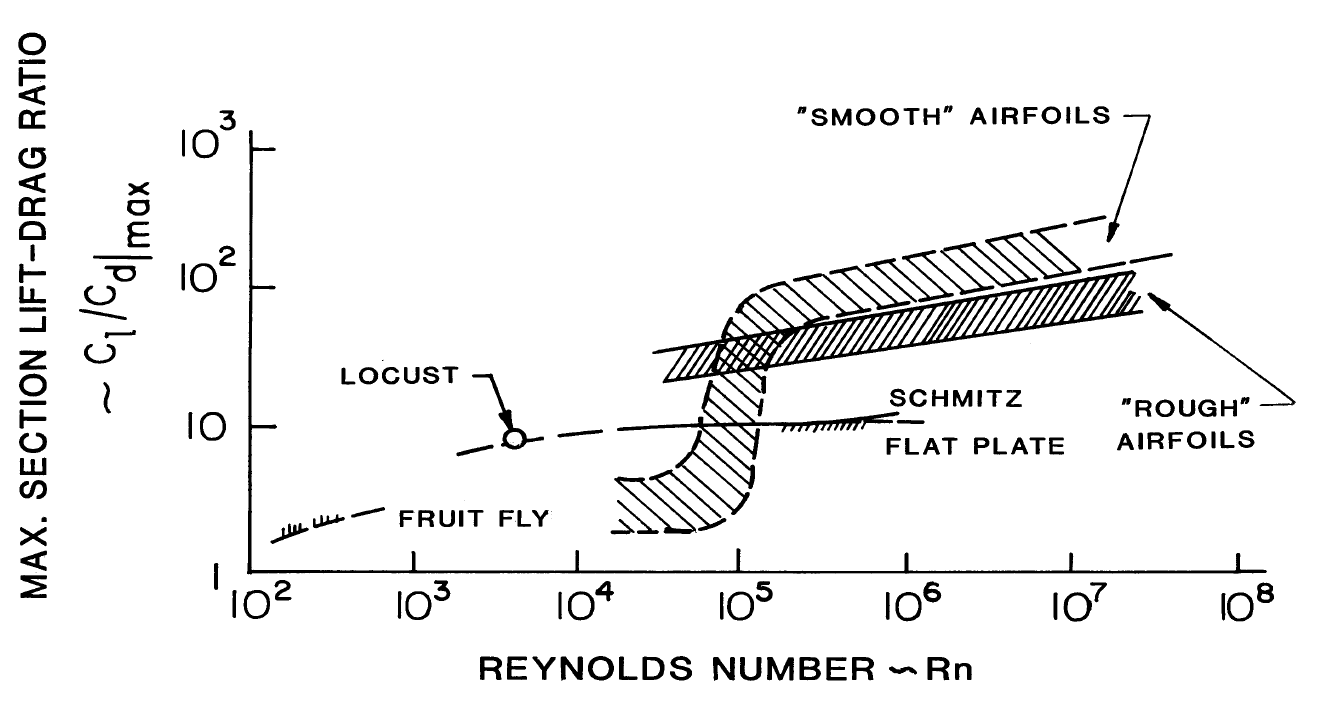
\includegraphics[width=0.7\textwidth]{figures/McMasters-Henderson-1980}

\caption{Airfoil maximum lift to drag ratio versus Reynolds number, from
    \cite{McMasters1980}.}

\label{fig:McMasters}
\end{figure}


\subsubsection{On Dynamic Foil Behavior}

Static foil performance does not tell the whole story for a cross-flow turbine.
The azimuthal, and therefore temporal variation of $\alpha$ in a cross-flow
turbine implies dynamic loading. Furthermore, since the range of angle of attack
encountered by a rotating blade increases with decreasing tip speed ratio, the
blades commonly undergo dynamic stall for tip speed ratios at and below those of
maximum rotor torque \cite{Para2002}. We then must understand the effects of
Reynolds number on the dynamic stall process.

Bousman \cite{Bousman2000-evaluation} states that dynamic stall is relatively
insensitive to Reynolds number for $Re=1.0 \times 10^5$--$2.5 \times
10^5$---judging from measurements on a pitching VR-7 foil in a wind and water
tunnel---since the loading is dominated by vortex shedding. However, Singleton
and Yeager Jr. \cite{Singleton2000} state that Reynolds number effects on
dynamic stall remains an unsolved question.


\subsubsection{On Wake Flows}

We expect that lower lift on the blades at lower $Re$ will weaken tip vortex
shedding, and decrease the levels of turbulence shed from the blade boundary
layers. As mentioned previously, the dynamic stall vortex shedding is not
expected to have a large Reynolds number sensitivity, though a larger separation
bubble at lower $Re$ may induce higher levels of turbulence as shed vortices
become unstable and break down.

Chamorro et al. \cite{Chamorro2012} showed that turbulence statistics in an AFT
wake became $Re$-independent at $Re_D \approx 1 \times 10^5$, and that mean
velocity profiles became $Re$-independent slightly earlier at $Re_D \approx 5
\times 10^4$. Note that in this study the tip chord Reynolds number was not
reported, but is estimated to be $Re_c \approx 4 \times 10^4$ at $Re_D=1 \times
10^5$.


\section{Experimental Setup}

Experiments were performed in a turbine test bed specifically designd for
cross-flow turbines. The turbine model used in this study was the UNH Reference
Vertical Axis Turbine (RVAT), which was designed to be a generic case for
numerical model testing, similar to the Sandia National Labs/US Department of
Energy RM2 River Turbine \cite{Neary2014}, but with higher solidity, or blade
chord to radius ratio.

The UNH-RVAT turbine has three blades made from NACA 0020 profiles with 0.140 m
chord. The blades are mounted at mid-chord w.r.t. the turbine axis, and the
turbine has a height (blade span) of 1 m and a diameter of 1 m, c.f.
Figure~\ref{fig:turbine}. The turbine test bed allows precise control and
measurement of the turbine shaft angle and angular velocity, and therefore tip
speed ratio, through a permanent magnet servo motor. The primary torque
measurement was provided by an in-line torque cell, with a redundant measurement
by a moment arm and load cell and an indirect measurement through the motor via
its torque constant. The turbine was mounted with in a low-drag frame
constructed from NACA 0020 foil sections.  The frame is attached to the tow
carriage by four linear bearings, allowing the total streamwise drag force to be
measured by a pair of S-beam load cells. Turbine rotor drag is calculated by
subtracting the test bed tare drag. A schematic of the turbine test bed is shown
in Figure~\ref{fig:exp-setup}. Additional details of the turbine and
experimental setup are described in \cite{Bachant2015-JoT}, and a CAD model of
the turbine is available from \cite{Bachant2014-RVAT-CAD}.

\begin{figure}[ht!]
\centering

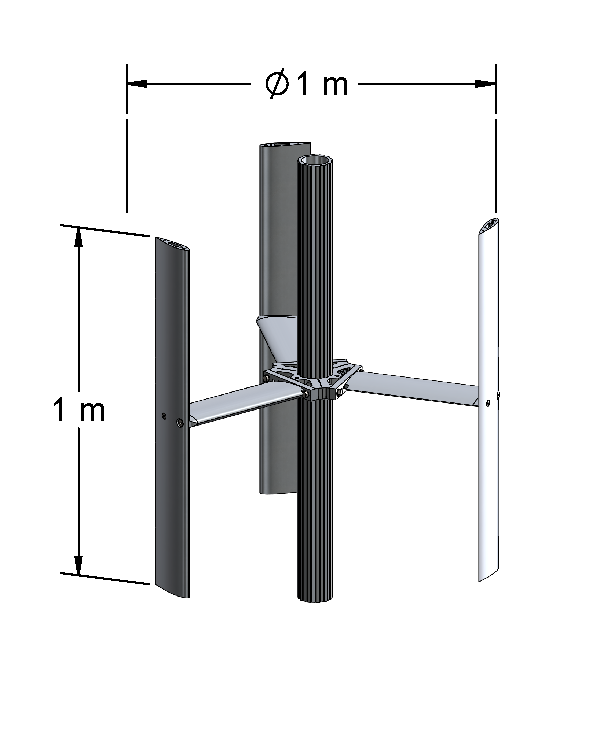
\includegraphics[width=0.4\textwidth]{figures/turbine}

\caption{UNH-RVAT turbine model. Turbine blades and struts made from NACA 0020
    profiles with 0.140 m chord. Note that the upper and lower mounting flanges have
    been excluded as these were included in the tare drag measurements.}

\label{fig:turbine}
\end{figure}


The turbine was mounted in a frame constructed from NACA 0020 sections. The
turbine shaft ran up through the water surface, coupled to a permanent magnet
servo motor with a 20:1 gearbox. This servo was controlled by the tow tank's
main motion controller for high synchronization with the carriage motion. A
rotary torque transducer was installed inline between the servo and the turbine,
and the servo was also mounted on a slewing ring bearing, which allowed a
redundant measurement of torque via an arm and load cell used to counteract the
turbine moment. The frame was mounted to the carriage via linear guides, such
that the total streamwise drag force was transferred to a pair of S-beam load
cells, providing the rotor drag measurements, after a measured tare drag was
subtracted in post processing. Similarly, a tare torque was measured by rotating
the turbine shaft in air. Turbine angular and tow carriage linear position were
measured using quadrature encoder signals, with $10^5$ counts-per-rev for the
turbine and 10 $\mathrm{\mu m}$ resolution for the carriage position. These
signals, along with the torque and drag signals, were sampled at 2 kHz.

\begin{figure}[ht!]
\centering
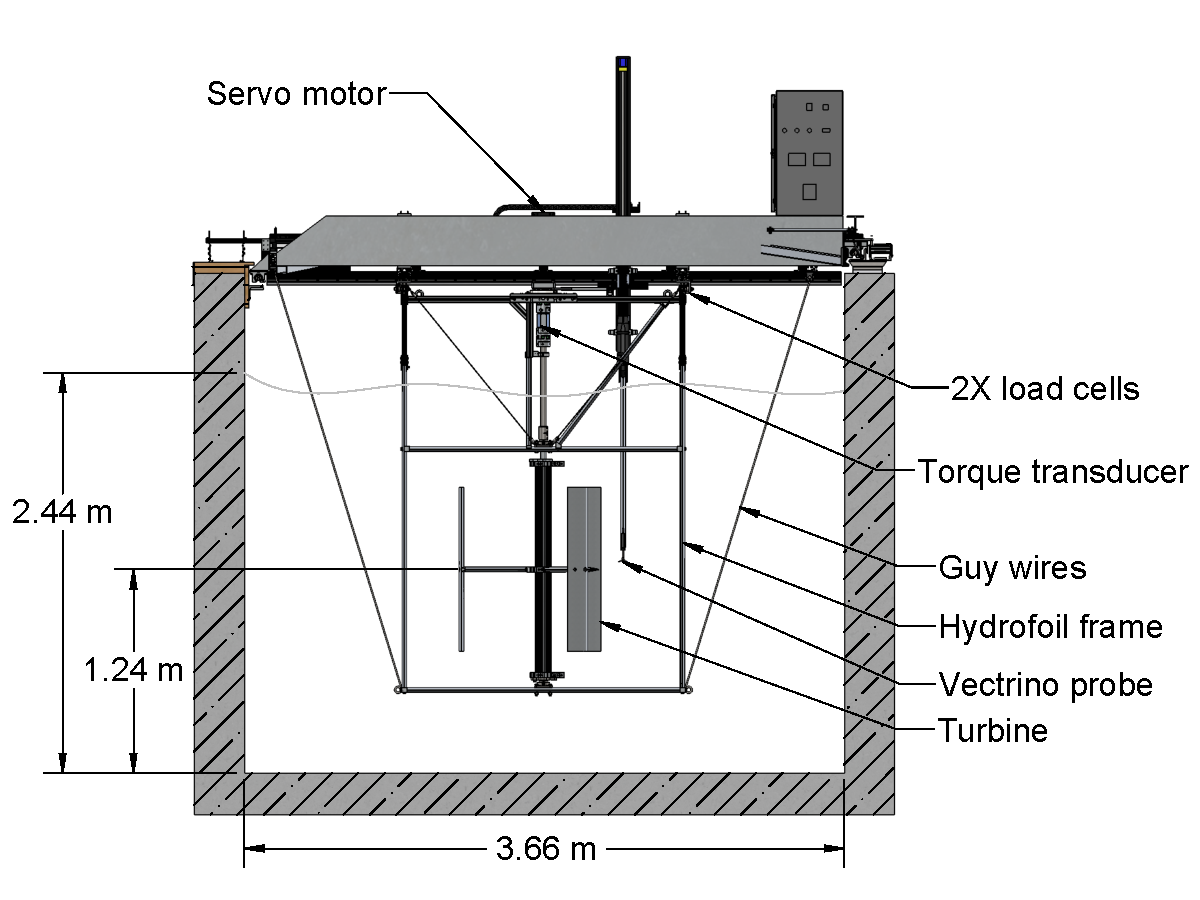
\includegraphics[width=0.75\textwidth]{figures/exp_setup_drawing}
\caption{Experimental setup: turbine test bed installed in UNH tow tank.}
\label{fig:exp-setup}
\end{figure}

Wake velocity was measured using a Nortek Vectrino+ acoustic Doppler velocimeter
(ADV), sampling at 200 Hz. The probe was mounted on an automated positioning
system, also controlled by the tow tank's main motion controller. The ADV and
DAQ systems' sampling times were synchronized by triggering the start of data
acquisition via a pulse sent from the motion controller.


\subsection{Test Plan}

Approximately 1500 tows were conducted for the study reported here, each tow was
used for a single data point on either a performance curve or wake map. Each
performance curve consisted of 31 tows, where during each tow the mean turbine
tip speed ratio was held constant, ranging from 0.1--3.1 in 0.1 increments. Full
performance curve data were acquired for tow speeds from 0.4 to 1.2 m/s in 0.2
m/s increments, for which turbine diameter and approximate blade chord Reynolds
number are presented in Table~\ref{tab:Re}. Performance was also measured for
$\lambda=1.9$ at tow speeds $[0.3, 0.5, 0.7, 0.9, 1.1, 1.3]$ m/s for two tows
each.

\begin{table}
\centering
\begin{tabular}{ccc}
Tow speed (m/s) & $Re_D$ & $Re_{c,\mathrm{ave}}$ ($\lambda = 1.9$) \\
\hline
0.3 & $3.0 \times 10^5$ & $8.0 \times 10^4$ \\
0.4 & $4.0 \times 10^5$ & $1.1 \times 10^5$ \\
0.5 & $5.0 \times 10^5$ & $1.3 \times 10^5$ \\
0.6 & $6.0 \times 10^5$ & $1.6 \times 10^5$ \\
0.7 & $7.0 \times 10^5$ & $1.9 \times 10^5$ \\
0.8 & $0.8 \times 10^5$ & $2.1 \times 10^5$ \\
0.9 & $0.9 \times 10^5$ & $2.4 \times 10^5$ \\
1.0 & $1.0 \times 10^6$ & $2.7 \times 10^5$ \\
1.1 & $1.1 \times 10^6$ & $2.9 \times 10^5$ \\
1.2 & $1.2 \times 10^6$ & $3.2 \times 10^5$ \\
1.3 & $1.3 \times 10^6$ & $3.4 \times 10^5$ \\
\end{tabular}
\caption{Turbine diameter and approximate blade chord Reynolds numbers for the
tow speeds used in the experiment.}
\label{tab:Re}
\end{table}

Each wake map was generated by positioning a Nortek Vectrino+ acoustic Doppler
Velocimeter (ADV), measuring three components of velocity at 200 Hz sampling
frequency, at 270 different locations, varied in the cross-stream and vertical
directions at one turbine diameter downstream ($x/D=1$). These locations have
vertical coordinates from the turbine centerline up to $z/H=0.625$, ranging in
the cross-stream direction $y/R = \pm 3$. These locations are shown in
Figure~\ref{fig:wake-locations}.


\begin{figure}
\centering
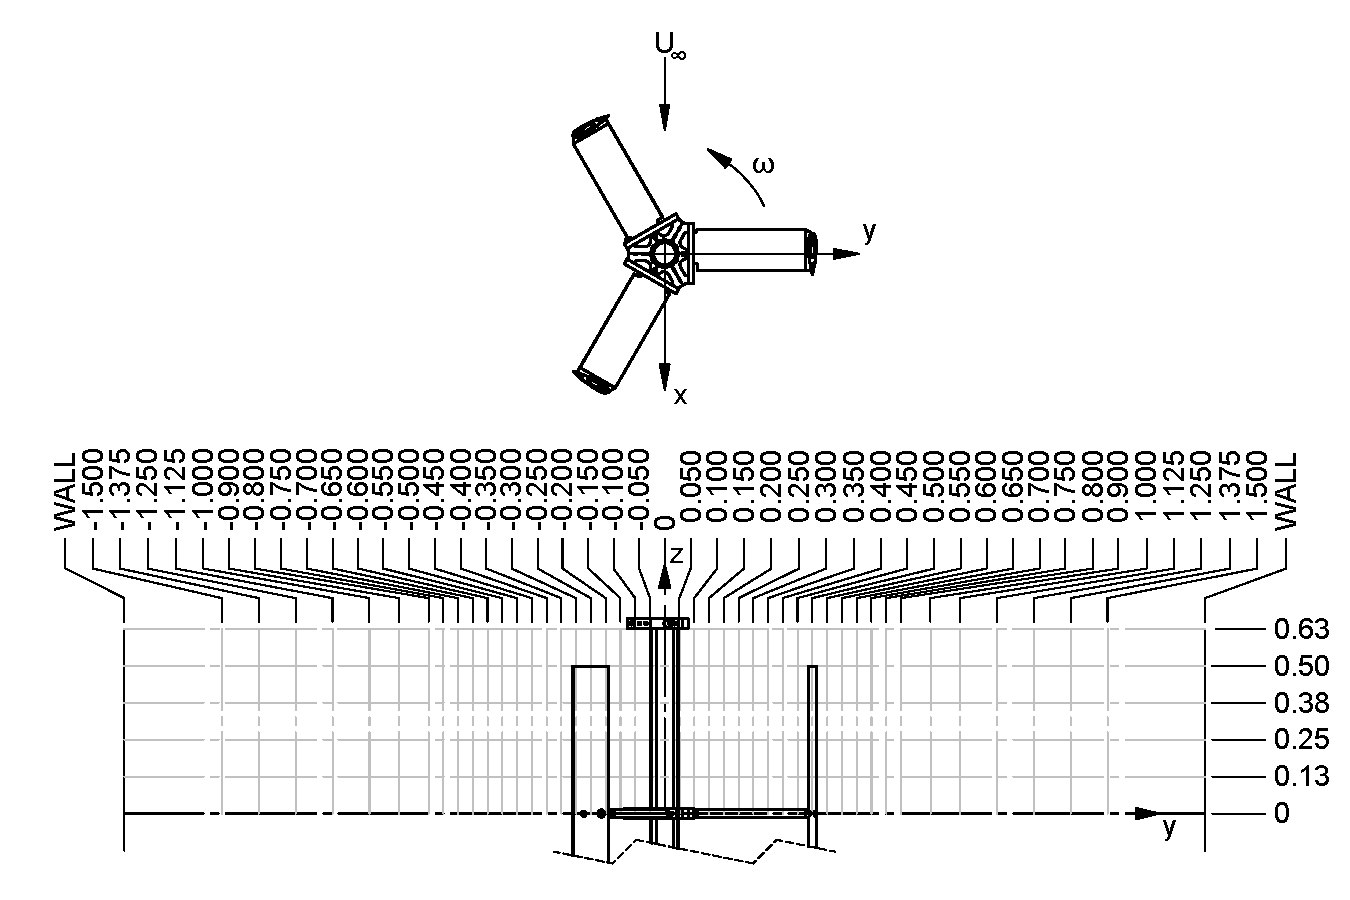
\includegraphics[width=0.9\textwidth]{figures/turbine_coordinate_system}
\caption{Wake measurement coordinate system and locations. Dimensions are in
meters.}
\label{fig:wake-locations}
\end{figure}


\subsection{Data Processing}

From each set of tows, a standard time interval was set, which allowed the
turbine performance and wake to reach a quasi-periodic state. Each run was
analyzed to compute statistics over this interval, truncating the end slightly
to achieve and integer number of blade passages. Turbine shaft angular velocity
and tow carriage speed were calculated using as second order central
differencing scheme on the respective position measurements. Power and drag
coefficients are calculated as instantaneous quantities using the carriage speed
as the free stream velocity.

Wake velocity data were filtered for spurious ``spikes'' by removing datapoints
8 standard deviations or 0.9 m/s from the mean. The experimental data and code
for processing and visualization are available from
\cite{Bachant2015-RVAT-Re-dep-data}.


\section{Results and Discussion}


\subsection{Performance}

Full power and rotor drag (a.k.a. thrust) coefficient curves for various
Reynolds numbers are plotted in Figure~\ref{fig:cp-curves} and
Figure~\ref{fig:cd-curves}, respectively. In general, maximum $C_P$ increases
with Reynolds number, which is due to an increase in the foil lift-to-drag
ratio. The power coefficient curves also show a slight downward shift in the
optimal tip speed ratio (peak performance) with increasing Reynolds number, from
about $\lambda \approx$ 2.0 to 1.9. This is caused by the stall delay from a
more turbulent boundary later on the blade suction side. There is essentially no
change in the shape of the drag coefficient curves---merely an upward shift in
$C_D$ with increasing $Re$.

\begin{figure}[ht]
\centering
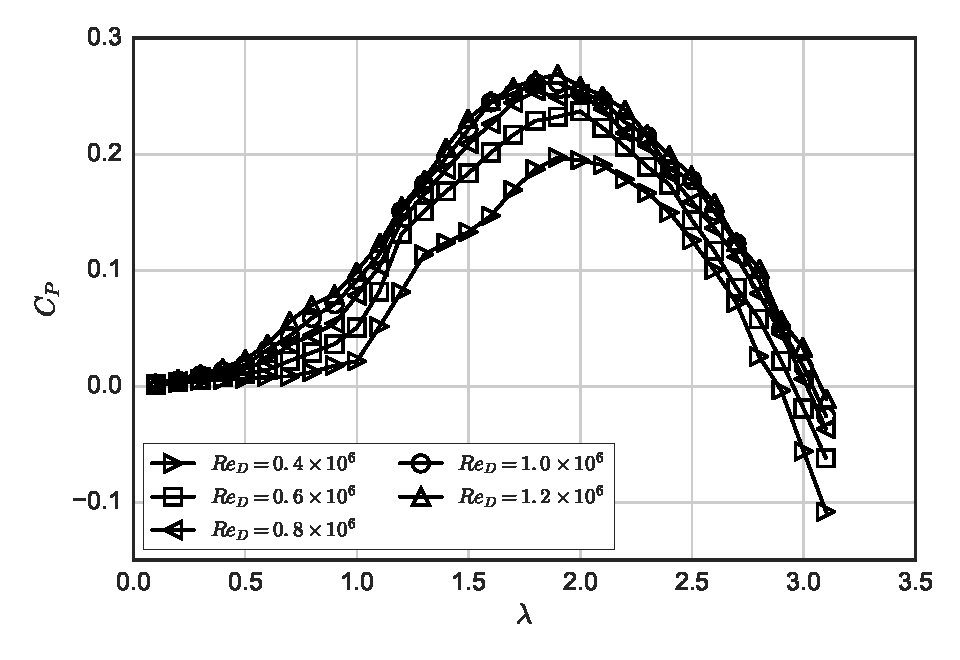
\includegraphics[width=0.65\textwidth]{figures/cp_curves}
\caption{Mean power coefficient curves plotted for
multiple Reynolds numbers.}
\label{fig:cp-curves}
\end{figure}

\begin{figure}[ht]
\centering
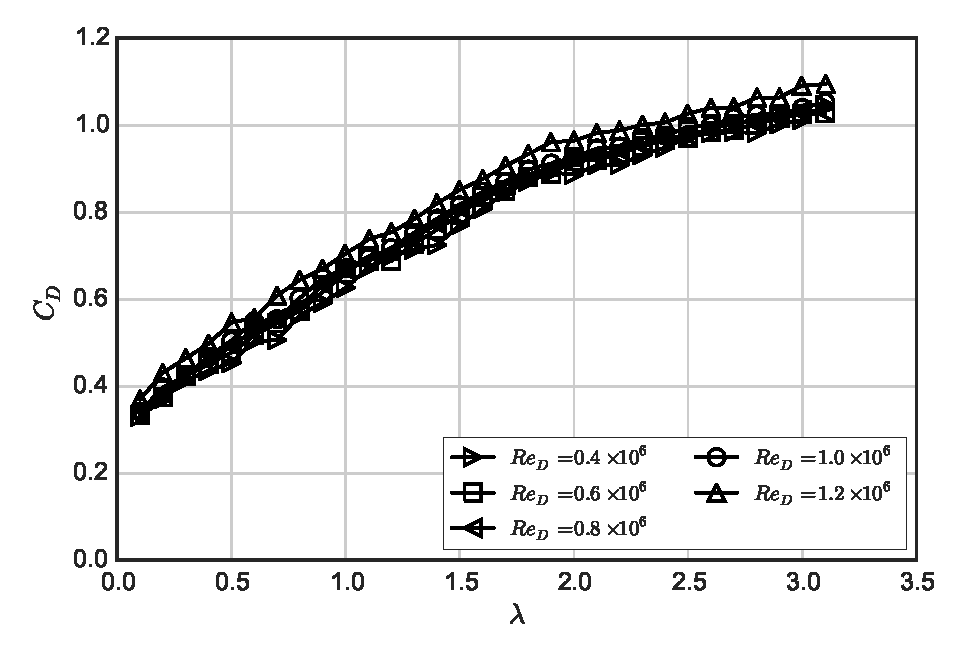
\includegraphics[width=0.65\textwidth]{figures/cd_curves}
\caption{Mean rotor drag coefficient curves plotted for
multiple Reynolds numbers.}
\label{fig:cd-curves}
\end{figure}

Mean power and drag coefficients at $\lambda=1.9$ are plotted versus Reynolds
number in Figure~\ref{fig:perf-Re-dep}. There is a drastic improvement in $C_P$
with increasing Reynolds number at lower values of Reynolds number. The power
coefficient then becomes  essentially $Re$-independent at $Re_D = 0.8 \times
10^6$, which corresponds to an approximate average blade chord Reynolds number
$Re_{c, \mathrm{ave}} = 2.1 \times 10^5$. This threshold is consistent with the
behavior of the blade boundary layer transitioning from laminar to turbulent,
thereby promoting either the suppression or reattachment of the laminar
separation bubble \cite{Lissaman1983}.

The behavior of the mean rotor drag coefficient is similar, though the changes
are less dramatic. This is likely due to cross-flow turbine geometry, where
increases in blade drag at lower $Re$ somewhat offsets the reduction in lift, to
keep total streamwise force from changing as much as the rotor torque. The
tendency for $C_D$ to continue increasing with $Re$ may also be a consequence of
increasing Froude number, which therefore increases free surface deformation and
wave drag during towing without increasing flow through the turbine.

\begin{figure}[ht]
\centering

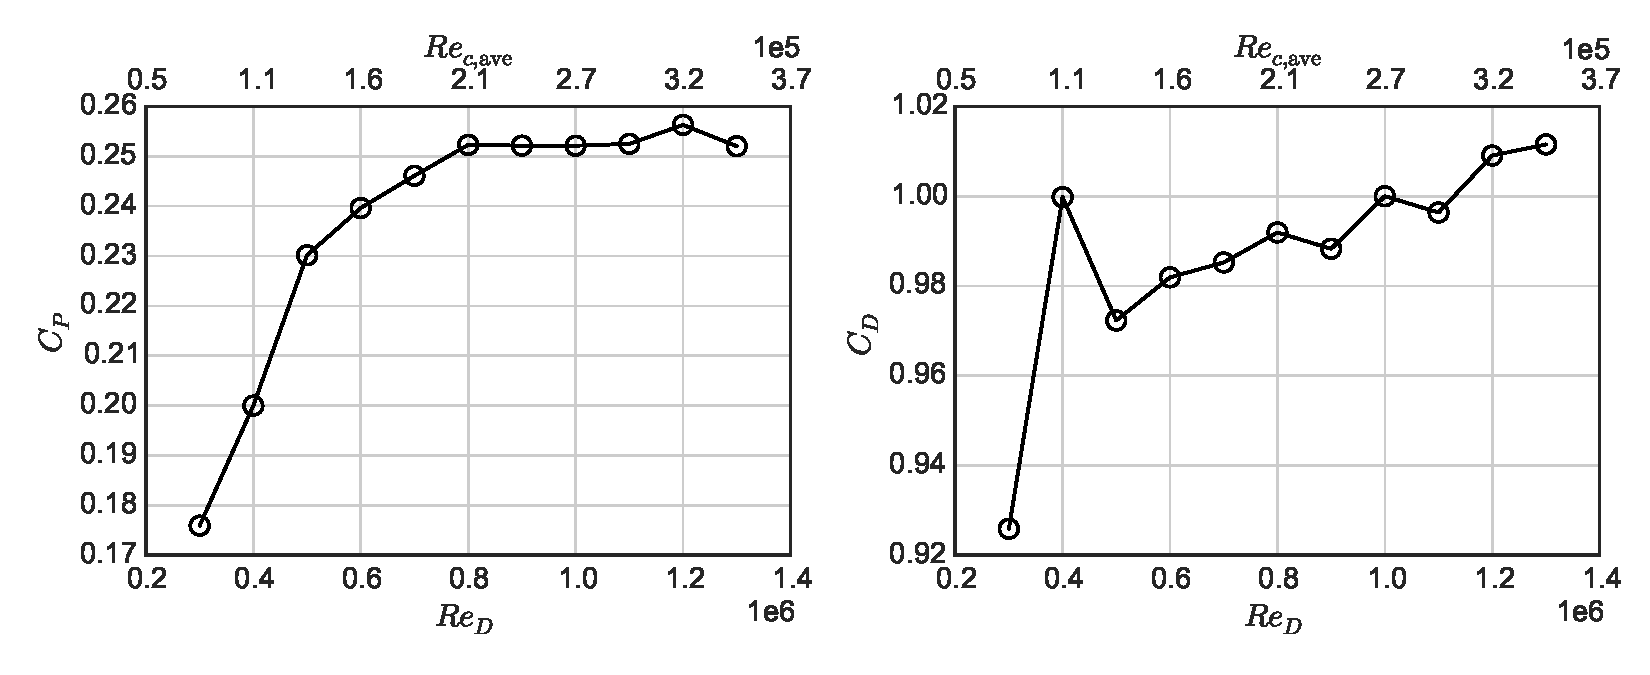
\includegraphics[width=0.9\textwidth]{figures/perf_re_dep}

\caption{UNH-RVAT measured mean power (left) and drag (right) coefficients at
    $\lambda=1.9$ plotted versus Reynolds number.}

\label{fig:perf-Re-dep}
\end{figure}


\subsubsection{Relation to Static Foil Characteristics}

To help understand---and possibly predict---the $Re$-sensitivity on turbine
performance, a series of static foil coefficient datasets were computed with the
XFOIL viscous panel method code \cite{Drela1989}, a commonly used tool for
airfoil analysis, e.g. \cite{Castelli2011, Walker2014}, implemented as part of
the open source turbine design software QBlade \cite{Marten2013}. Simulations
were run for an angle of attack range of 0--40 degrees, in increments of 0.5
degrees. Solver parameters used a 100 panels, a fixed speed, zero Mach number,
\texttt{NCrit=9} (default $\mathrm{e}^n$ transition criteria parameter for an
average wind tunnel), and no forced boundary layer transition. Characteristics
were computed for the approximate average blade chord Reynolds numbers
encountered in the tow tank experiments.

To investigate the effects of the blades' ``virtual camber'' due to their
circular path \cite{Migliore1980}, the XFOIL calculations were performed for
20\% thick foils with 0\% (NACA 0020), 2\% (NACA 2520), and 4\% (NACA 4520)
camber about their half-chord location. A 4\% camber approximates the maximum
distance between the blade chord line and path for the UNH-RVAT and the 2\%
camber takes into account the reduction in virtual flow curvature from the
non-curved inflow velocity by dividing by the tip speed ratio $\lambda=1.9$.

Results from the XFOIL calculations are shown in Figure~\ref{fig:foil-Re-dep},
where values of maximum lift coefficient, minimum drag coefficient, and maximum
lift-to-drag ratio are normalized (for comparison between foils) and plotted
versus $Re_c$. In general, larger camber is associated with decreased foil
performance at lower Reynolds number. The data and processing code for these
calculations is available from \cite{Bachant2015-NACAXX20-XFOIL}.

\begin{figure}[ht!]
\centering
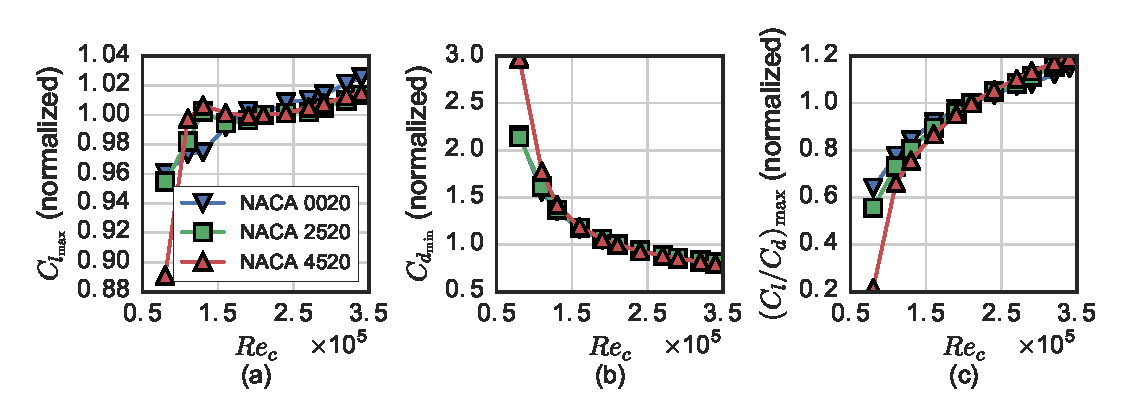
\includegraphics[width=0.9\textwidth]{figures/all_foils_re_dep}
\caption{Foil section characteristics computed by XFOIL for various $Re_c$.}
\label{fig:foil-Re-dep}
\end{figure}

In conjunction with the cross-flow turbine blade kinematics, the foil
coefficients were used to approximate turbine performance by calculating the
peak torque coefficient on the upstream half of the blade path. The turbine
torque coefficient $C_T$ can be related to the blade section chordwise force
coefficient $C_c$ by
\begin{equation}
C_T = \frac{C_c c}{2R} \frac{|U_\mathrm{rel}|^2}{U_\infty^2},
\end{equation}
where the blade section chordwise force (for zero preset pitch) is given by
\begin{equation}
C_c = C_l \sin \alpha - C_d \cos \alpha.
\end{equation}

The relative blade velocity $U_\mathrm{rel}$ was calculated by vector addition
of the free stream velocity and the opposite of the blade tangential velocity.
Note that this neglects any induction, or slowing of the free stream by the
turbine forces, which would be present in a momentum/streamtube model. Since the
goal of this approach was not to predict absolute performance but rather gain
insight into relative changes with $Re$, this method was deemed acceptable as it
is extremely simple and fast to compute.

Values for the blade angle of attack, relative velocity, and torque coefficient
are plotted in Figure~\ref{fig:blade-kinematics} for the upstream half of
rotation of the turbine. The effects of static stall are clearly present in the
torque coefficient plot, and by the time the angle of attack has decreased below
that of stall, the relative velocity is so low that there is not much
contribution to the torque coefficient.

\begin{figure}[ht!]
\centering

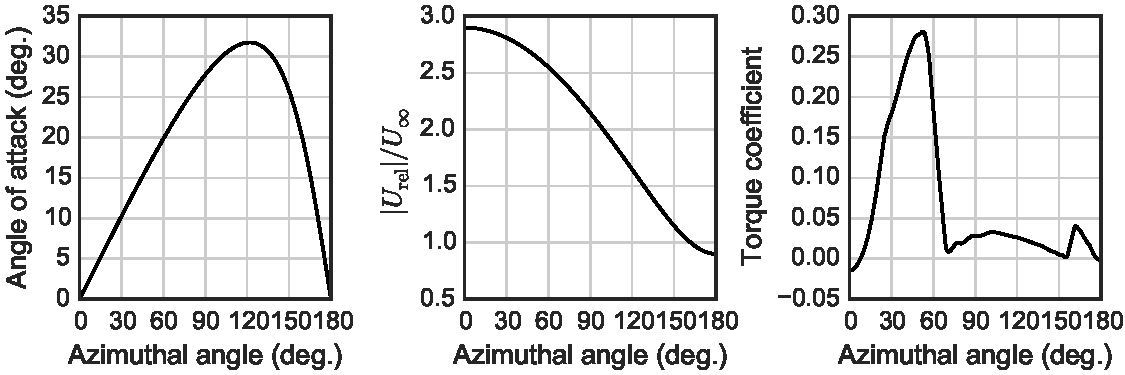
\includegraphics[width=0.9\textwidth]{figures/foil_kinematics_ct}

\caption{Geometric angle of attack, relative velocity and torque coefficient
    calculated with a NACA 0020 foil operating at $\lambda=1.9$.}

\label{fig:blade-kinematics}
\end{figure}

Results for the normalized peak torque coefficient for each foil are plotted
versus $Re_c$ in Figure~\ref{fig:foils-C_T-Re-dep}. It is interesting that the
convergence of $C_{T_\mathrm{max}}$ with increasing Reynolds number is more
dramatic than any of the common foil performance characteristics plotted in
Figure~\ref{fig:foil-Re-dep}, meaning that the cross-flow turbine's unique
kinematics must be taken into account when attempting to predict the effect of
transitional Reynolds numbers on turbine performance.

From the peak torque coefficient metric, the Reynolds number independence is
achieved at lower values, and more dramatically. We see that the trend of the
(non-cambered) NACA 0020 curve matches almost perfectly up to $Re_c \approx 2.1
\times 10^5$, but then continues to increase linearly with a small slope with
$Re$. This is not matched by the experimental data, which at higher $Re$ looks
more like the cambered foil results. Though this method is very approximate, it
nevertheless appears to be a reasonable way to predict the transitional Reynolds
number regime for cross-flow turbine performance using only 2-D static airfoil
characteristics

\begin{figure}[ht!]
\centering

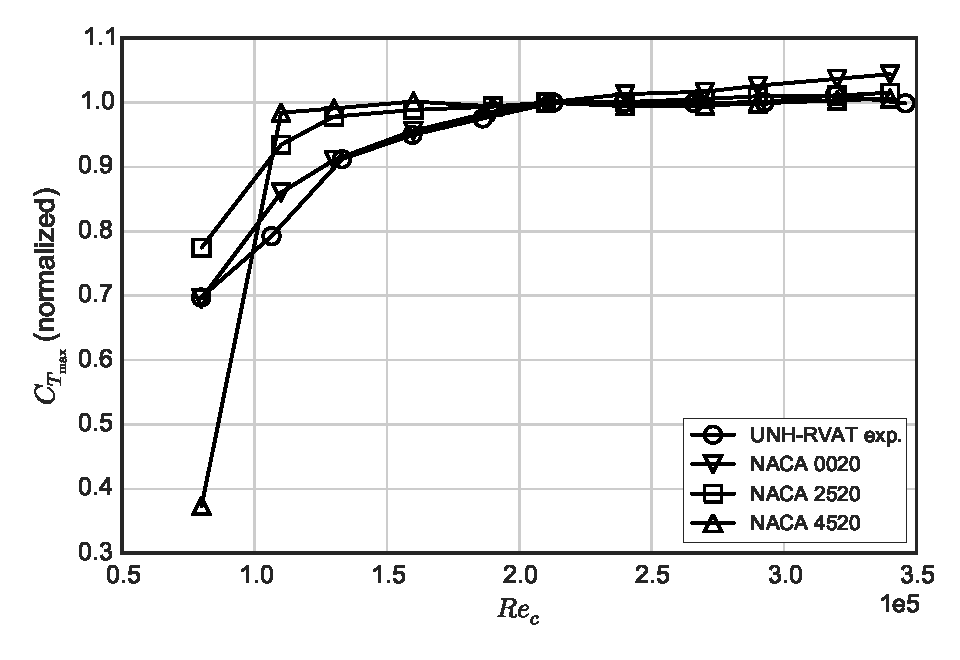
\includegraphics[width=0.65\textwidth]{figures/cft_re_dep_foils}

\caption{Reynolds number dependence of the normalized peak torque coefficient
    calculated from static foil coefficients and blade kinematics, compared to
    experimental data from a cross-flow turbine. Note that the experimental data
    represents the mean torque coefficient, not the maximum.}

\label{fig:foils-C_T-Re-dep}
\end{figure}


\subsection{Wake Characteristics}

The near-wake of this turbine at $x/D=1$, $\lambda=1.9$, and momentum and
kinetic energy balances at a $Re_D = 1.0 \times 10^6$ were discussed in
\cite{Bachant2015-JoT}. Similar data were taken for the experiment here, and
results for the mean velocity field and turbulence kinetic energy calculated
from wake maps of 270 individual measurements (tows) are shown in
Figure~\ref{fig:meancontquiv} and Figure~\ref{fig:kcont}, respectively, looking
upstream towards the turbine. With respect to the mean velocity field, we see
asymmetry and a mean vortex structure created by blade tip vortex shedding. The
effects of the tip vortices are also seen in the turbulence kinetic energy
measurements, along with turbulence generated by the blades undergoing dynamic
stall on the $-y$ side of the turbine.

These same wake maps were measured for $Re_D = 0.4 \times 10^6$, $0.6 \times
10^6$, $0.8 \times 10^6$, and $1.2 \times 10^6$. Qualitatively, these look
strikingly similar, so they have not been plotted here. We will instead compare
and contrast the wake behavior by examining spectra and wake transport terms in
the equations that govern the downstream evolution of mean momentum and kinetic
energy.

\begin{figure}[ht!]
\centering
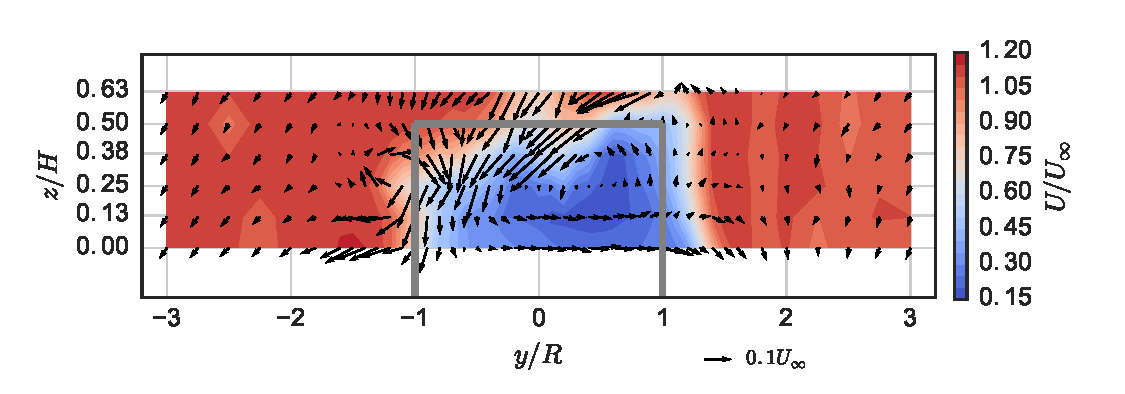
\includegraphics[width=0.8\textwidth]{figures/meancontquiv_10}
\caption{Mean velocity field at $x/D=1$, $\lambda=1.9$, and $Re_D=1.0 \times 10^6$.}
\label{fig:meancontquiv}
\end{figure}

\begin{figure}[ht!]
\centering
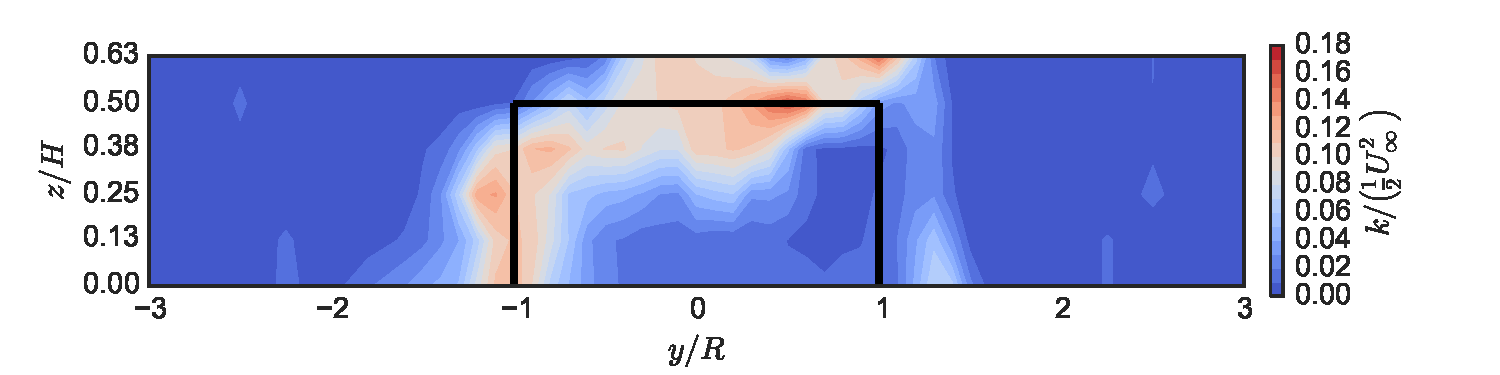
\includegraphics[width=0.8\textwidth]{figures/k_contours_10}
\caption{Turbulence kinetic energy at $x/D=1$, $\lambda=1.9$, and
$Re_D=1.0 \times 10^6$.}
\label{fig:kcont}
\end{figure}


\subsubsection{Dominant Timescales and Turbulence Spectra}

Spectra of the cross-stream velocity normalized by the free stream are plotted
in Figure~\ref{fig:wake-spectra} for regions on either side of the turbine. On
the $-y$ side of the turbine there is broadband turbulence produced by blade
stall, and on the $+y$ side there is a clear peak in the spectra caused by the
blade passage. We see that on both sides there is higher spectral energy at
lower Reynolds numbers. On the $+y$ side of the turbine we notice higher
spectral energy at the blade passage frequency's first harmonic, or $6
f_\mathrm{turbine}$. This is likely due to the blade's shed vorticity being less
stable at higher $Re$.

\begin{figure}[ht!]
\centering

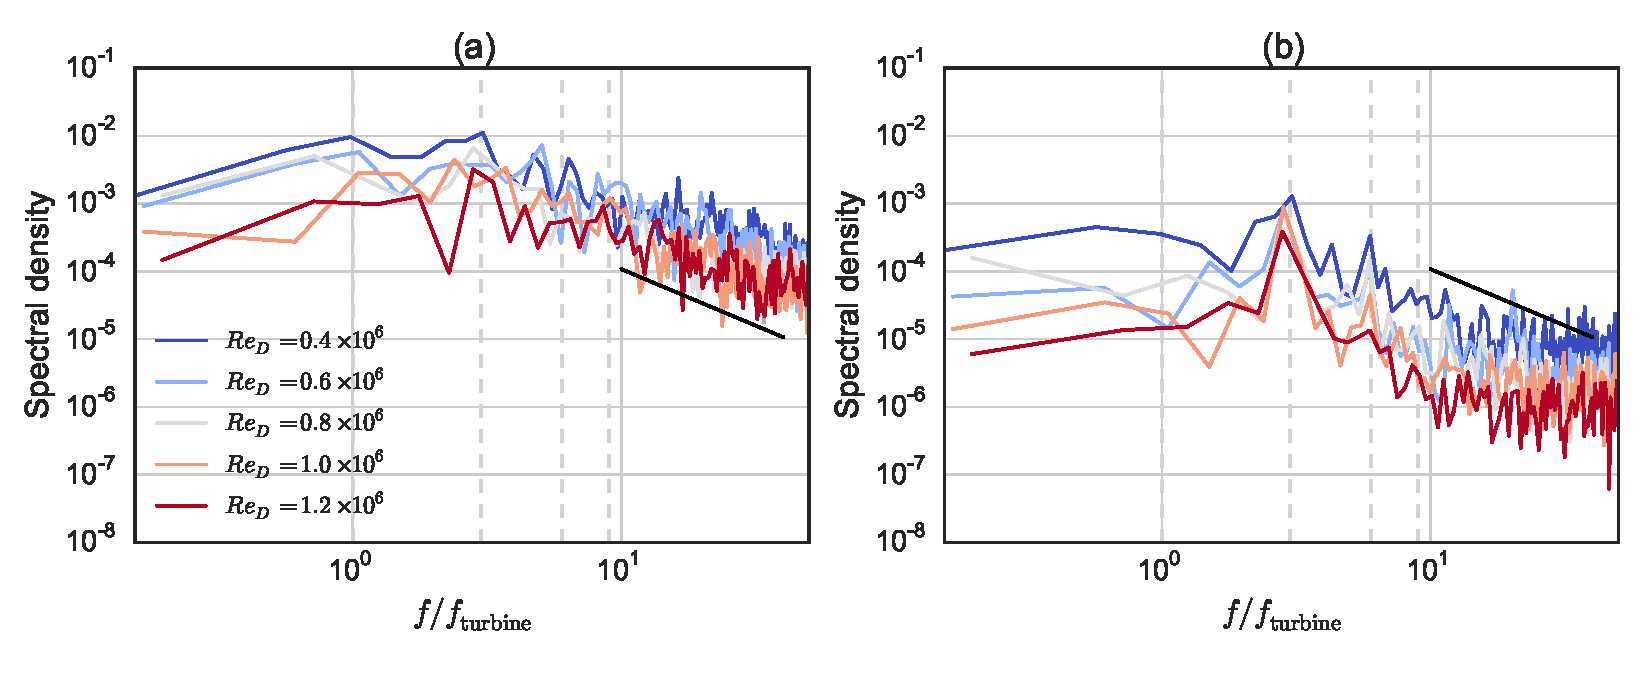
\includegraphics[width=0.85\textwidth]{figures/wake_spectra}

\caption{Cross-stream velocity (normalized by $U_\infty$) spectra at $z/H=0.25$,
    $y/R=-1.0$ ($-0.5$ m in Figure~\ref{fig:wake-locations}) (a) and $y/R=1.5$
    ($+0.75$ m in Figure~\ref{fig:wake-locations}) (b). Dashed vertical lines
    indicate $[1, 3, 6, 9]$ times the turbine rotational frequency.}

\label{fig:wake-spectra}
\end{figure}



\subsubsection{Transport of Mean Momentum and Kinetic Energy}

The relative importance of various physical processes on mean streamwise
momentum and kinetic energy transport/recovery in the streamwise direction are
plotted in Figures~\ref{fig:mom-bar-graph} and \ref{fig:K-bar-graph},
respectively. We note that similar to \cite{Bachant2015-JoT}, the vertical
advection at this point in the wake is the dominant contributor to positive wake
recovery, caused by the unique vortex pattern created by the blade tips and
wakes.

We see that in general, levels of turbulent transport are slightly lower at
larger Reynolds numbers. The viscous diffusion and dissipation, though still
three orders of magnitude smaller than the other terms, do increase at low
Reynolds numbers, which is consistent with the physical meaning of the Reynolds
number in general. From these results one might expect that the viscous effects
will become significant to the wake dynamics around $Re_D \sim 10^4$.

\begin{figure}[ht!]
\centering
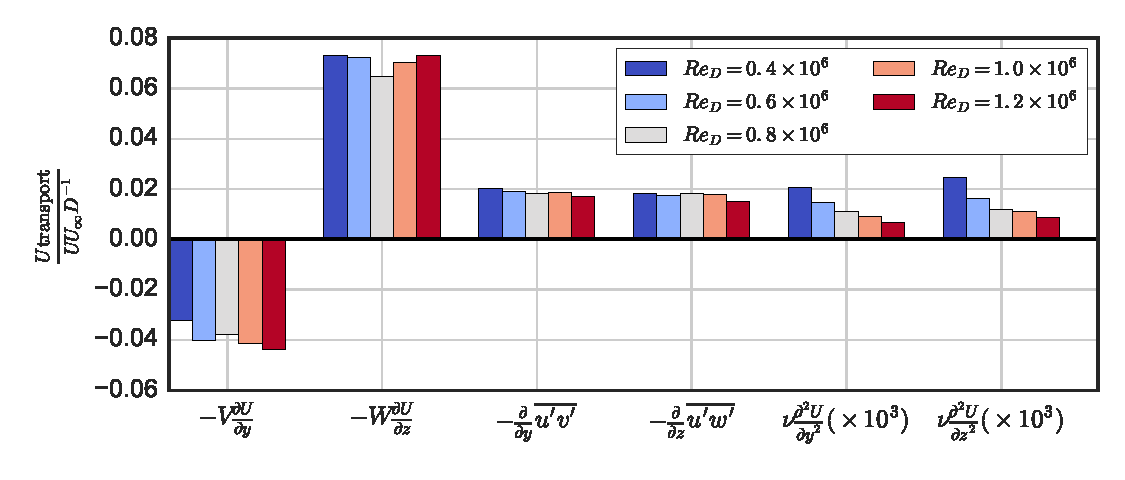
\includegraphics[width=0.9\textwidth]{figures/mom_bar_graph}
\caption{Momentum transport quantities.}
\label{fig:mom-bar-graph}
\end{figure}

\begin{figure}[ht!]
\centering
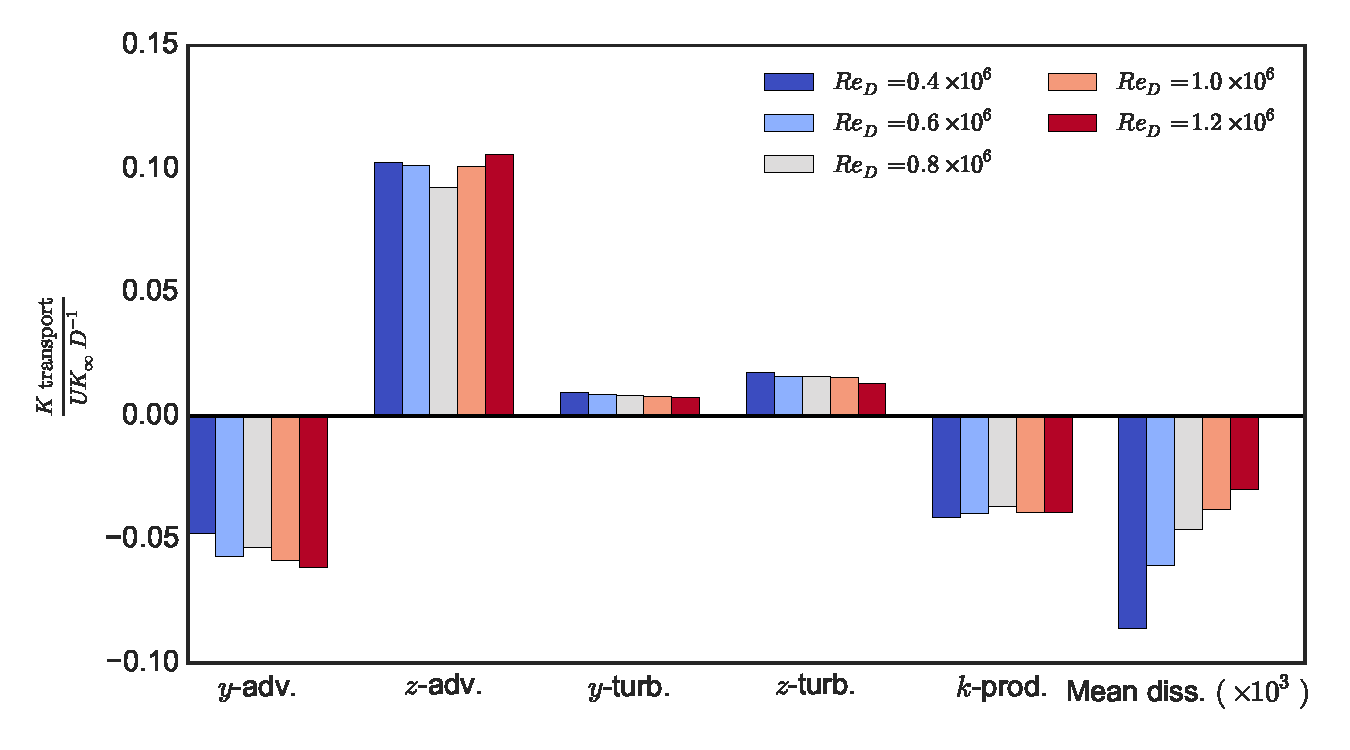
\includegraphics[width=0.9\textwidth]{figures/K_trans_bar_graph}
\caption{Mean kinetic energy transport quantities.}
\label{fig:K-bar-graph}
\end{figure}

The totals for all the wake transport terms calculated in
Figures~\ref{fig:mom-bar-graph} and \ref{fig:K-bar-graph} are plotted in
Figure~\ref{fig:wake-trans-totals}. We see that in general wake transport of
both mean streamwise momentum and kinetic energy is enhanced at lower Reynolds
numbers and levels off consistent with the behavior of the turbine power
coefficient. This is an important consideration if studying sub-scale models of
turbine arrays, where increased levels of wake recovery could motivate different
ideal array configurations when compared with full-scale turbines if the scale
model Reynolds number is too low.

\begin{figure}[ht!]
\centering
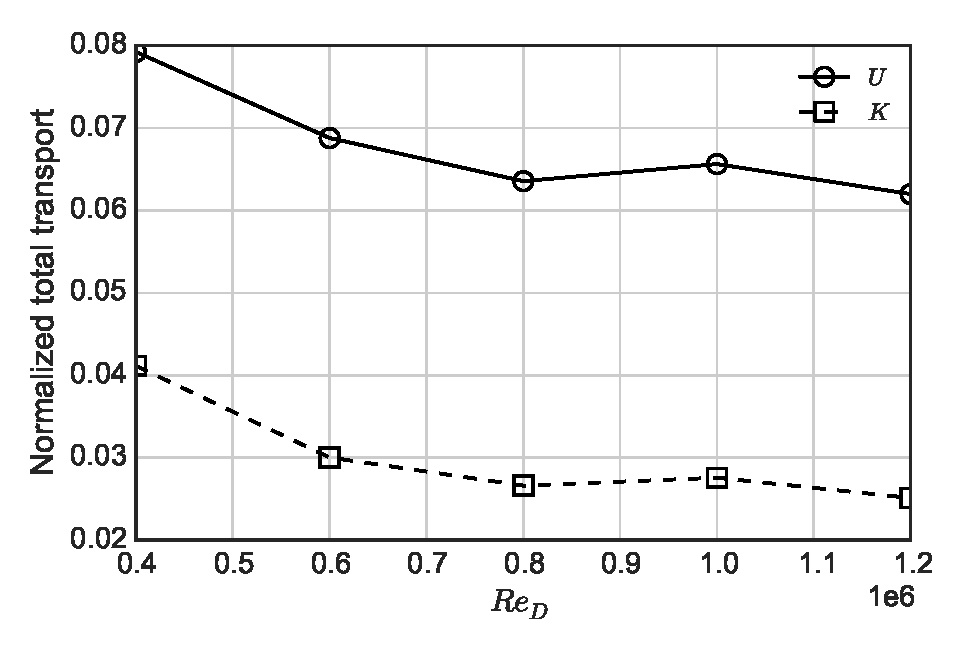
\includegraphics[width=0.65\textwidth]{figures/wake_trans_totals}
\caption{Normalized transport totals from Figures~\ref{fig:mom-bar-graph} and
\ref{fig:K-bar-graph} plotted versus Reynolds number.}
\label{fig:wake-trans-totals}
\end{figure}


\section{Conclusions}

In this study it was demonstrated that the performance of a high solidity
($c/R=0.28$) cross-flow turbine becomes essentially $Re$-independent at a
Reynolds number based on turbine diameter of $Re_D \approx 10^6$, or an
approximate Reynolds number based on blade chord of $Re_c \approx 2 \times
10^5$.

\todo[inline]{Issues such as blade termination/strength of tip vortices?}

These results suggest that to validate predictive engineering models, one must
use data of at least this scale, especially for validation of high-fidelity CFD
models, where transition to turbulence may be completely different between
scaled physical model and full-scale prototype.

We propose a method for predicting Reynolds number dependence of a cross-flow
turbine using static airfoil characteristics and turbine blade kinematics. It is
shown that the peak torque coefficient computed this way shows similar Reynolds
number sensitivity---a better predictor than conventional quantifications of
airfoil performance, e.g., lift-to-drag ratio. The simple peak geometric torque
coefficient model predicted Reynolds number independence for Reynolds numbers
based on blade chord of $Re_c > 2 \times 10^5$. Is it also shown from this
metric that foils with higher camber are more Reynolds number dependent but have
smaller slopes in the linear regime. The Reynolds number dependence of the peak
torque coefficient calculated from static foil data and cross-flow turbine
kinematics was shown to be a reasonable indicator for predicting Reynolds number
dependence of an actual cross-flow turbine operating under dynamic conditions,
including dynamic stall.

If using scaled physical models to predict array performance, it is important to
keep all turbines in the regime where the power coefficient varies linearly to
avoid exaggerated power deficiencies for downstream turbines, despite
similarities in wake characteristics. These results also suggest that low
Reynolds number physical model studies of turbine arrays may see exaggerated
levels of wake recovery, leading to inadequate or inappropriate spacing or
layouts.


\acknowledgements{Acknowledgements}

The authors would like to acknowledge funding through a National Science
Foundation CAREER award (PI Wosnik, NSF-CBET 1150797, program manager Dr. Ram
Gupta), a grant through the Leslie S. Hubbard Marine Program Endowment to
purchase acoustic flow measurement instrumentation, and a grant for laboratory
infrastructure upgrades through the US Department of Energy.

\conflictofinterests{Conflicts of Interest}

The authors declare no conflict of interest.


\bibliography{library}
\bibliographystyle{mdpi}

\end{document}
